\documentclass[]{article}
\usepackage{lmodern}
\usepackage{amssymb,amsmath}
\usepackage{ifxetex,ifluatex}
\usepackage{fixltx2e} % provides \textsubscript
\ifnum 0\ifxetex 1\fi\ifluatex 1\fi=0 % if pdftex
  \usepackage[T1]{fontenc}
  \usepackage[utf8]{inputenc}
\else % if luatex or xelatex
  \ifxetex
    \usepackage{mathspec}
  \else
    \usepackage{fontspec}
  \fi
  \defaultfontfeatures{Ligatures=TeX,Scale=MatchLowercase}
\fi
% use upquote if available, for straight quotes in verbatim environments
\IfFileExists{upquote.sty}{\usepackage{upquote}}{}
% use microtype if available
\IfFileExists{microtype.sty}{%
\usepackage{microtype}
\UseMicrotypeSet[protrusion]{basicmath} % disable protrusion for tt fonts
}{}
\usepackage[margin=1in]{geometry}
\usepackage{hyperref}
\hypersetup{unicode=true,
            pdftitle={ANOVA pedagogica \textasciitilde{} unidade},
            pdfauthor={Geiser C. Challco geiser@usp.br},
            pdfborder={0 0 0},
            breaklinks=true}
\urlstyle{same}  % don't use monospace font for urls
\usepackage{color}
\usepackage{fancyvrb}
\newcommand{\VerbBar}{|}
\newcommand{\VERB}{\Verb[commandchars=\\\{\}]}
\DefineVerbatimEnvironment{Highlighting}{Verbatim}{commandchars=\\\{\}}
% Add ',fontsize=\small' for more characters per line
\usepackage{framed}
\definecolor{shadecolor}{RGB}{248,248,248}
\newenvironment{Shaded}{\begin{snugshade}}{\end{snugshade}}
\newcommand{\AlertTok}[1]{\textcolor[rgb]{0.94,0.16,0.16}{#1}}
\newcommand{\AnnotationTok}[1]{\textcolor[rgb]{0.56,0.35,0.01}{\textbf{\textit{#1}}}}
\newcommand{\AttributeTok}[1]{\textcolor[rgb]{0.77,0.63,0.00}{#1}}
\newcommand{\BaseNTok}[1]{\textcolor[rgb]{0.00,0.00,0.81}{#1}}
\newcommand{\BuiltInTok}[1]{#1}
\newcommand{\CharTok}[1]{\textcolor[rgb]{0.31,0.60,0.02}{#1}}
\newcommand{\CommentTok}[1]{\textcolor[rgb]{0.56,0.35,0.01}{\textit{#1}}}
\newcommand{\CommentVarTok}[1]{\textcolor[rgb]{0.56,0.35,0.01}{\textbf{\textit{#1}}}}
\newcommand{\ConstantTok}[1]{\textcolor[rgb]{0.00,0.00,0.00}{#1}}
\newcommand{\ControlFlowTok}[1]{\textcolor[rgb]{0.13,0.29,0.53}{\textbf{#1}}}
\newcommand{\DataTypeTok}[1]{\textcolor[rgb]{0.13,0.29,0.53}{#1}}
\newcommand{\DecValTok}[1]{\textcolor[rgb]{0.00,0.00,0.81}{#1}}
\newcommand{\DocumentationTok}[1]{\textcolor[rgb]{0.56,0.35,0.01}{\textbf{\textit{#1}}}}
\newcommand{\ErrorTok}[1]{\textcolor[rgb]{0.64,0.00,0.00}{\textbf{#1}}}
\newcommand{\ExtensionTok}[1]{#1}
\newcommand{\FloatTok}[1]{\textcolor[rgb]{0.00,0.00,0.81}{#1}}
\newcommand{\FunctionTok}[1]{\textcolor[rgb]{0.00,0.00,0.00}{#1}}
\newcommand{\ImportTok}[1]{#1}
\newcommand{\InformationTok}[1]{\textcolor[rgb]{0.56,0.35,0.01}{\textbf{\textit{#1}}}}
\newcommand{\KeywordTok}[1]{\textcolor[rgb]{0.13,0.29,0.53}{\textbf{#1}}}
\newcommand{\NormalTok}[1]{#1}
\newcommand{\OperatorTok}[1]{\textcolor[rgb]{0.81,0.36,0.00}{\textbf{#1}}}
\newcommand{\OtherTok}[1]{\textcolor[rgb]{0.56,0.35,0.01}{#1}}
\newcommand{\PreprocessorTok}[1]{\textcolor[rgb]{0.56,0.35,0.01}{\textit{#1}}}
\newcommand{\RegionMarkerTok}[1]{#1}
\newcommand{\SpecialCharTok}[1]{\textcolor[rgb]{0.00,0.00,0.00}{#1}}
\newcommand{\SpecialStringTok}[1]{\textcolor[rgb]{0.31,0.60,0.02}{#1}}
\newcommand{\StringTok}[1]{\textcolor[rgb]{0.31,0.60,0.02}{#1}}
\newcommand{\VariableTok}[1]{\textcolor[rgb]{0.00,0.00,0.00}{#1}}
\newcommand{\VerbatimStringTok}[1]{\textcolor[rgb]{0.31,0.60,0.02}{#1}}
\newcommand{\WarningTok}[1]{\textcolor[rgb]{0.56,0.35,0.01}{\textbf{\textit{#1}}}}
\usepackage{longtable,booktabs}
\usepackage{graphicx,grffile}
\makeatletter
\def\maxwidth{\ifdim\Gin@nat@width>\linewidth\linewidth\else\Gin@nat@width\fi}
\def\maxheight{\ifdim\Gin@nat@height>\textheight\textheight\else\Gin@nat@height\fi}
\makeatother
% Scale images if necessary, so that they will not overflow the page
% margins by default, and it is still possible to overwrite the defaults
% using explicit options in \includegraphics[width, height, ...]{}
\setkeys{Gin}{width=\maxwidth,height=\maxheight,keepaspectratio}
\IfFileExists{parskip.sty}{%
\usepackage{parskip}
}{% else
\setlength{\parindent}{0pt}
\setlength{\parskip}{6pt plus 2pt minus 1pt}
}
\setlength{\emergencystretch}{3em}  % prevent overfull lines
\providecommand{\tightlist}{%
  \setlength{\itemsep}{0pt}\setlength{\parskip}{0pt}}
\setcounter{secnumdepth}{0}
% Redefines (sub)paragraphs to behave more like sections
\ifx\paragraph\undefined\else
\let\oldparagraph\paragraph
\renewcommand{\paragraph}[1]{\oldparagraph{#1}\mbox{}}
\fi
\ifx\subparagraph\undefined\else
\let\oldsubparagraph\subparagraph
\renewcommand{\subparagraph}[1]{\oldsubparagraph{#1}\mbox{}}
\fi

%%% Use protect on footnotes to avoid problems with footnotes in titles
\let\rmarkdownfootnote\footnote%
\def\footnote{\protect\rmarkdownfootnote}

%%% Change title format to be more compact
\usepackage{titling}

% Create subtitle command for use in maketitle
\providecommand{\subtitle}[1]{
  \posttitle{
    \begin{center}\large#1\end{center}
    }
}

\setlength{\droptitle}{-2em}

  \title{ANOVA \texttt{pedagogica} \textasciitilde{} \texttt{unidade}}
    \pretitle{\vspace{\droptitle}\centering\huge}
  \posttitle{\par}
    \author{Geiser C. Challco \href{mailto:geiser@usp.br}{\nolinkurl{geiser@usp.br}}}
    \preauthor{\centering\large\emph}
  \postauthor{\par}
    \date{}
    \predate{}\postdate{}
  

\begin{document}
\maketitle

\begin{itemize}
\tightlist
\item
  Report as Word format: \url{factorialAnova.docx}
\item
  Report as LaTex format: \url{factorialAnova.tex}
\end{itemize}

\hypertarget{initial-data-and-preprocessing}{%
\subsection{Initial Data and
Preprocessing}\label{initial-data-and-preprocessing}}

R script: \url{factorialAnova.R} Inital data: \url{data.csv}

\hypertarget{visualization-of-data-distribution}{%
\subsubsection{Visualization of data
distribution}\label{visualization-of-data-distribution}}

\begin{Shaded}
\begin{Highlighting}[]
\KeywordTok{ggdensity}\NormalTok{(dat, }\DataTypeTok{x =} \StringTok{"pedagogica"}\NormalTok{, }\DataTypeTok{fill =} \StringTok{"lightgray"}\NormalTok{, }\DataTypeTok{title=} \StringTok{"Density of pedagogica before transformation"}\NormalTok{) }\OperatorTok{+}
\StringTok{ }\KeywordTok{stat_overlay_normal_density}\NormalTok{(}\DataTypeTok{color =} \StringTok{"red"}\NormalTok{, }\DataTypeTok{linetype =} \StringTok{"dashed"}\NormalTok{)}
\end{Highlighting}
\end{Shaded}

\includegraphics{factorialAnova_files/figure-latex/unnamed-chunk-1-1.pdf}

\hypertarget{dealing-with-positive-greater-skewness-in-pedagogica}{%
\subsubsection{Dealing with positive greater skewness in
pedagogica}\label{dealing-with-positive-greater-skewness-in-pedagogica}}

\begin{Shaded}
\begin{Highlighting}[]
\NormalTok{dat[[}\StringTok{"pedagogica"}\NormalTok{]] <-}\StringTok{ }\KeywordTok{log10}\NormalTok{(dat[[}\StringTok{"pedagogica"}\NormalTok{]])}
\end{Highlighting}
\end{Shaded}

\begin{Shaded}
\begin{Highlighting}[]
\KeywordTok{ggdensity}\NormalTok{(dat, }\DataTypeTok{x =} \StringTok{"pedagogica"}\NormalTok{, }\DataTypeTok{fill =} \StringTok{"lightgray"}\NormalTok{, }\DataTypeTok{title=} \StringTok{"Density of pedagogica after transformation"}\NormalTok{) }\OperatorTok{+}
\StringTok{ }\KeywordTok{stat_overlay_normal_density}\NormalTok{(}\DataTypeTok{color =} \StringTok{"red"}\NormalTok{, }\DataTypeTok{linetype =} \StringTok{"dashed"}\NormalTok{)}
\end{Highlighting}
\end{Shaded}

\includegraphics{factorialAnova_files/figure-latex/unnamed-chunk-3-1.pdf}

\hypertarget{summary-statistics-of-the-initial-data}{%
\subsubsection{Summary statistics of the initial
data}\label{summary-statistics-of-the-initial-data}}

\begin{Shaded}
\begin{Highlighting}[]
\KeywordTok{get_summary_stats}\NormalTok{(}\KeywordTok{group_by}\NormalTok{(dat, }\StringTok{`}\DataTypeTok{unidade}\StringTok{`}\NormalTok{), }\DataTypeTok{type =}\StringTok{"common"}\NormalTok{)}
\end{Highlighting}
\end{Shaded}

\begin{verbatim}
## # A tibble: 3 x 11
##   unidade   variable     n   min   max median   iqr  mean    sd    se    ci
##   <fct>     <chr>    <dbl> <dbl> <dbl>  <dbl> <dbl> <dbl> <dbl> <dbl> <dbl>
## 1 UFAL A.C~ pedagog~   241 0     0.699  0.301 0.342 0.302 0.191 0.012 0.024
## 2 UFAL Ara~ pedagog~    55 0     0.699  0.243 0.301 0.25  0.186 0.025 0.05 
## 3 UFAL CECA pedagog~    24 0.097 0.628  0.243 0.263 0.313 0.156 0.032 0.066
\end{verbatim}

\hypertarget{check-assumptions}{%
\subsection{Check Assumptions}\label{check-assumptions}}

\hypertarget{identifying-outliers}{%
\subsubsection{Identifying outliers}\label{identifying-outliers}}

Outliers tend to increase type-I error probability, and they decrease
the calculated F statistic in ANOVA resulting in a lower chance of
reject the null hypothesis.

\begin{itemize}
\tightlist
\item
  Identified outliers using rstatix
\end{itemize}

\begin{Shaded}
\begin{Highlighting}[]
\KeywordTok{identify_outliers}\NormalTok{(}\KeywordTok{group_by}\NormalTok{(dat, }\StringTok{`}\DataTypeTok{unidade}\StringTok{`}\NormalTok{), }\StringTok{`}\DataTypeTok{pedagogica}\StringTok{`}\NormalTok{)}
\end{Highlighting}
\end{Shaded}

\begin{verbatim}
## [1] unidade    ID         pedagogica is.outlier is.extreme
## <0 rows> (or 0-length row.names)
\end{verbatim}

\begin{itemize}
\tightlist
\item
  Identified outliers through Boxplots
\end{itemize}

\begin{Shaded}
\begin{Highlighting}[]
\KeywordTok{Boxplot}\NormalTok{(}\StringTok{`}\DataTypeTok{pedagogica}\StringTok{`} \OperatorTok{~}\StringTok{ `}\DataTypeTok{unidade}\StringTok{`}\NormalTok{, }\DataTypeTok{data =}\NormalTok{ dat, }\DataTypeTok{id =} \KeywordTok{list}\NormalTok{(}\DataTypeTok{n =} \OtherTok{Inf}\NormalTok{))}
\end{Highlighting}
\end{Shaded}

\includegraphics{factorialAnova_files/figure-latex/unnamed-chunk-6-1.pdf}

\hypertarget{removing-outliers-from-the-data}{%
\subsubsection{Removing outliers from the
data}\label{removing-outliers-from-the-data}}

\begin{Shaded}
\begin{Highlighting}[]
\NormalTok{outliers <-}\StringTok{ }\KeywordTok{c}\NormalTok{(}\StringTok{""}\NormalTok{)}
\NormalTok{rdat <-}\StringTok{ }\NormalTok{dat[}\OperatorTok{!}\NormalTok{dat[[}\StringTok{"ID"}\NormalTok{]] }\OperatorTok\StringTok{ }\NormalTok{outliers,]   }\CommentTok{# table without outliers}
\end{Highlighting}
\end{Shaded}

\begin{longtable}[]{@{}llr@{}}
\caption{Outliers table}\tabularnewline
\toprule
ID & unidade & pedagogica\tabularnewline
\midrule
\endfirsthead
\toprule
ID & unidade & pedagogica\tabularnewline
\midrule
\endhead
\bottomrule
\end{longtable}

\hypertarget{normality-assumption}{%
\subsubsection{Normality assumption}\label{normality-assumption}}

\textbf{Observation}:

As sample sizes increase, ANOVA remains a valid test even with the
violation of normality {[}\protect\hyperlink{references}{1},
\protect\hyperlink{references}{2}{]}. According to the central limit
theorem, the sampling distribution tends to be normal if the sample is
large enough (\texttt{n\ \textgreater{}\ 30}). Therefore, we performed
ANOVA with large samples as follows:

\begin{itemize}
\item
  In cases with the sample size greater than 30
  (\texttt{n\ \textgreater{}\ 30}), we adopted a significance level of
  \texttt{p\ \textless{}\ 0.01} instead a significance level of
  \texttt{p\ \textless{}\ 0.05}.
\item
  For samples with \texttt{n\ \textgreater{}\ 50} observation, we
  adopted D'Agostino-Pearson test that offers better accuracy for larger
  samples {[}\protect\hyperlink{references}{3}{]}.
\item
  For samples' size between \texttt{n\ \textgreater{}\ 100} and
  \texttt{n\ \textless{}=\ 200}, we ignored both tests (Shapiro and
  D'Agostino-Persons), and our decision of normality were based only in
  the interpretation of QQ-plots and histograms because these tests tend
  to be too sensitive with values greater than 200
  {[}\protect\hyperlink{references}{3}{]}.
\item
  For samples with \texttt{n\ \textgreater{}\ 200} observation, we
  ignore the normality assumption based on the central theorem limit,
  and taking only into account the homogeneity assumption.
\end{itemize}

\hypertarget{checking-normality-assumption-in-the-residual-model}{%
\paragraph{Checking normality assumption in the residual
model}\label{checking-normality-assumption-in-the-residual-model}}

\begin{Shaded}
\begin{Highlighting}[]
\NormalTok{mdl <-}\StringTok{ }\KeywordTok{lm}\NormalTok{(}\StringTok{`}\DataTypeTok{pedagogica}\StringTok{`} \OperatorTok{~}\StringTok{ `}\DataTypeTok{unidade}\StringTok{`}\NormalTok{, }\DataTypeTok{data =}\NormalTok{ rdat)}
\KeywordTok{normality_test}\NormalTok{(}\KeywordTok{residuals}\NormalTok{(mdl))}
\end{Highlighting}
\end{Shaded}

\begin{verbatim}
##     n statistic     method            p p.signif normality
## 1 320  54.94218 D'Agostino 1.173395e-12     ****         -
\end{verbatim}

The QQ plot used to evaluate normality assumption

\begin{Shaded}
\begin{Highlighting}[]
\KeywordTok{qqPlot}\NormalTok{(}\KeywordTok{residuals}\NormalTok{(mdl))}
\end{Highlighting}
\end{Shaded}

\includegraphics{factorialAnova_files/figure-latex/unnamed-chunk-10-1.pdf}

\begin{verbatim}
## Obs322 Obs188 
##    312    184
\end{verbatim}

\hypertarget{checking-normality-assumption-for-each-group}{%
\paragraph{Checking normality assumption for each
group}\label{checking-normality-assumption-for-each-group}}

\begin{Shaded}
\begin{Highlighting}[]
\KeywordTok{normality_test_at}\NormalTok{(}\KeywordTok{group_by}\NormalTok{(rdat, }\StringTok{`}\DataTypeTok{unidade}\StringTok{`}\NormalTok{), }\StringTok{"pedagogica"}\NormalTok{)}
\end{Highlighting}
\end{Shaded}

\begin{verbatim}
##                 variable          unidade   n  statistic       method
## 1             pedagogica UFAL A.C. Simões 241 57.5426659   D'Agostino
## Omnibus  Test pedagogica   UFAL Arapiraca  55  2.8290093   D'Agostino
## 11            pedagogica        UFAL CECA  24  0.9156624 Shapiro-Wilk
##                          p p.signif normality
## 1             3.197442e-13     ****         -
## Omnibus  Test 2.430460e-01       ns       YES
## 11            4.687579e-02        *        NO
\end{verbatim}

\begin{itemize}
\tightlist
\item
  QQ plot in the \textbf{unidade}: ``UFAL A.C. Simões''
\end{itemize}

\begin{Shaded}
\begin{Highlighting}[]
\KeywordTok{qqPlot}\NormalTok{( }\OperatorTok{~}\StringTok{ `}\DataTypeTok{pedagogica}\StringTok{`}\NormalTok{, }\DataTypeTok{data =}\NormalTok{ rdat[}\KeywordTok{which}\NormalTok{(rdat[}\StringTok{"unidade"}\NormalTok{] }\OperatorTok{==}\StringTok{ "UFAL A.C. Simões"),])}
\end{Highlighting}
\end{Shaded}

\includegraphics{factorialAnova_files/figure-latex/unnamed-chunk-12-1.pdf}

\begin{verbatim}
## Obs188 Obs234 
##    141    173
\end{verbatim}

\begin{itemize}
\tightlist
\item
  QQ plot in the \textbf{unidade}: ``UFAL Arapiraca''
\end{itemize}

\begin{Shaded}
\begin{Highlighting}[]
\KeywordTok{qqPlot}\NormalTok{( }\OperatorTok{~}\StringTok{ `}\DataTypeTok{pedagogica}\StringTok{`}\NormalTok{, }\DataTypeTok{data =}\NormalTok{ rdat[}\KeywordTok{which}\NormalTok{(rdat[}\StringTok{"unidade"}\NormalTok{] }\OperatorTok{==}\StringTok{ "UFAL Arapiraca"}\NormalTok{),])}
\end{Highlighting}
\end{Shaded}

\includegraphics{factorialAnova_files/figure-latex/unnamed-chunk-13-1.pdf}

\begin{verbatim}
## Obs322  Obs48 
##     54      7
\end{verbatim}

\begin{itemize}
\tightlist
\item
  QQ plot in the \textbf{unidade}: ``UFAL CECA''
\end{itemize}

\begin{Shaded}
\begin{Highlighting}[]
\KeywordTok{qqPlot}\NormalTok{( }\OperatorTok{~}\StringTok{ `}\DataTypeTok{pedagogica}\StringTok{`}\NormalTok{, }\DataTypeTok{data =}\NormalTok{ rdat[}\KeywordTok{which}\NormalTok{(rdat[}\StringTok{"unidade"}\NormalTok{] }\OperatorTok{==}\StringTok{ "UFAL CECA"}\NormalTok{),])}
\end{Highlighting}
\end{Shaded}

\includegraphics{factorialAnova_files/figure-latex/unnamed-chunk-14-1.pdf}

\begin{verbatim}
## Obs160 Obs166 
##      6      7
\end{verbatim}

\hypertarget{removing-data-that-affect-normality}{%
\paragraph{Removing data that affect
normality}\label{removing-data-that-affect-normality}}

\begin{Shaded}
\begin{Highlighting}[]
\NormalTok{non.normal <-}\StringTok{ }\KeywordTok{c}\NormalTok{(}\StringTok{"Obs111"}\NormalTok{,}\StringTok{"Obs239"}\NormalTok{)}
\NormalTok{sdat <-}\StringTok{ }\NormalTok{rdat[}\OperatorTok{!}\NormalTok{rdat[[}\StringTok{"ID"}\NormalTok{]] }\OperatorTok\StringTok{ }\NormalTok{non.normal,]   }\CommentTok{# table without non-normal and outliers}
\end{Highlighting}
\end{Shaded}

\begin{longtable}[]{@{}lllr@{}}
\caption{Non-normal data table}\tabularnewline
\toprule
& ID & unidade & pedagogica\tabularnewline
\midrule
\endfirsthead
\toprule
& ID & unidade & pedagogica\tabularnewline
\midrule
\endhead
Obs111 & Obs111 & UFAL CECA & 0.1760913\tabularnewline
Obs239 & Obs239 & UFAL CECA & 0.0969100\tabularnewline
\bottomrule
\end{longtable}

\hypertarget{performing-normality-test-without-data-that-affect-normality}{%
\paragraph{Performing normality test without data that affect
normality}\label{performing-normality-test-without-data-that-affect-normality}}

\begin{Shaded}
\begin{Highlighting}[]
\NormalTok{mdl <-}\StringTok{ }\KeywordTok{lm}\NormalTok{(}\StringTok{`}\DataTypeTok{pedagogica}\StringTok{`} \OperatorTok{~}\StringTok{ `}\DataTypeTok{unidade}\StringTok{`}\NormalTok{, }\DataTypeTok{data =}\NormalTok{ sdat)}
\KeywordTok{normality_test}\NormalTok{(}\KeywordTok{residuals}\NormalTok{(mdl))}
\end{Highlighting}
\end{Shaded}

\begin{longtable}[]{@{}rrllll@{}}
\toprule
n & statistic & method & p & p.signif & normality\tabularnewline
\midrule
\endhead
318 & 54.9806 & D'Agostino & \textless{} 0.0001 & **** &
-\tabularnewline
\bottomrule
\end{longtable}

\begin{Shaded}
\begin{Highlighting}[]
\KeywordTok{normality_test_at}\NormalTok{(}\KeywordTok{group_by}\NormalTok{(sdat, }\StringTok{`}\DataTypeTok{unidade}\StringTok{`}\NormalTok{), }\StringTok{"pedagogica"}\NormalTok{)}
\end{Highlighting}
\end{Shaded}

\begin{longtable}[]{@{}llrrllll@{}}
\toprule
variable & unidade & n & statistic & method & p & p.signif &
normality\tabularnewline
\midrule
\endhead
pedagogica & UFAL A.C. Simões & 241 & 57.5427 & D'Agostino & \textless{}
0.0001 & **** & -\tabularnewline
pedagogica & UFAL Arapiraca & 55 & 2.8290 & D'Agostino & 0.243 & ns &
YES\tabularnewline
pedagogica & UFAL CECA & 22 & 0.9191 & Shapiro-Wilk & 0.0727 & ns &
YES\tabularnewline
\bottomrule
\end{longtable}

QQ plot in the residual model without data that affect normality

\begin{Shaded}
\begin{Highlighting}[]
\KeywordTok{qqPlot}\NormalTok{(}\KeywordTok{residuals}\NormalTok{(mdl))}
\end{Highlighting}
\end{Shaded}

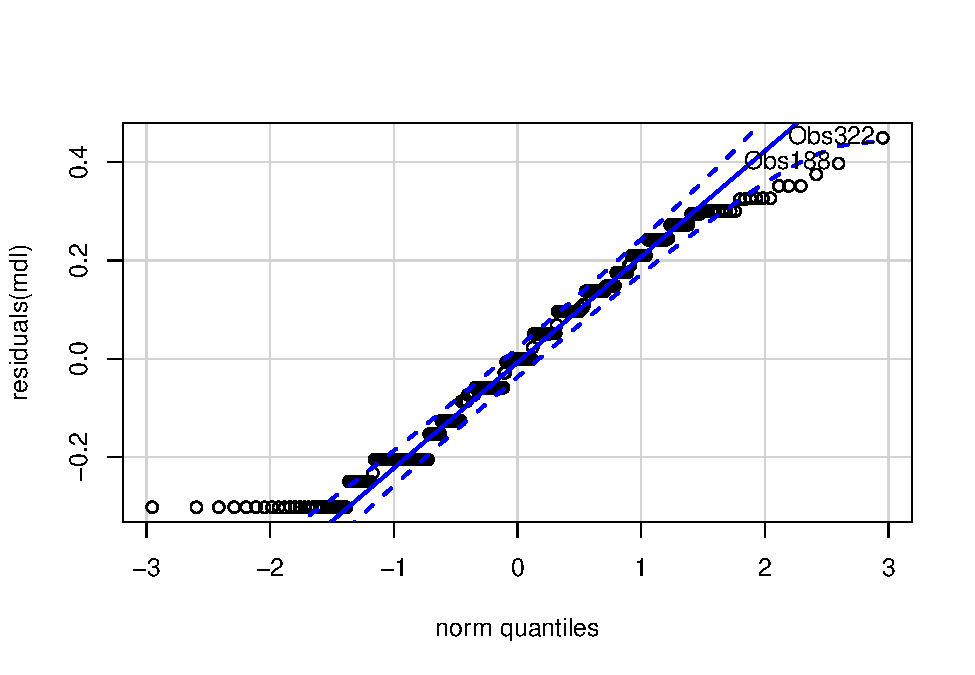
\includegraphics{factorialAnova_files/figure-latex/unnamed-chunk-19-1.pdf}

\begin{verbatim}
## Obs322 Obs188 
##    310    183
\end{verbatim}

\begin{itemize}
\tightlist
\item
  QQ plot in the \textbf{unidade}: ``UFAL A.C. Simões''
\end{itemize}

\begin{Shaded}
\begin{Highlighting}[]
\KeywordTok{qqPlot}\NormalTok{( }\OperatorTok{~}\StringTok{ `}\DataTypeTok{pedagogica}\StringTok{`}\NormalTok{, }\DataTypeTok{data =}\NormalTok{ sdat[}\KeywordTok{which}\NormalTok{(sdat[}\StringTok{"unidade"}\NormalTok{] }\OperatorTok{==}\StringTok{ "UFAL A.C. Simões"),])}
\end{Highlighting}
\end{Shaded}

\includegraphics{factorialAnova_files/figure-latex/unnamed-chunk-20-1.pdf}

\begin{verbatim}
## Obs188 Obs234 
##    141    173
\end{verbatim}

\begin{itemize}
\tightlist
\item
  QQ plot in the \textbf{unidade}: ``UFAL Arapiraca''
\end{itemize}

\begin{Shaded}
\begin{Highlighting}[]
\KeywordTok{qqPlot}\NormalTok{( }\OperatorTok{~}\StringTok{ `}\DataTypeTok{pedagogica}\StringTok{`}\NormalTok{, }\DataTypeTok{data =}\NormalTok{ sdat[}\KeywordTok{which}\NormalTok{(sdat[}\StringTok{"unidade"}\NormalTok{] }\OperatorTok{==}\StringTok{ "UFAL Arapiraca"}\NormalTok{),])}
\end{Highlighting}
\end{Shaded}

\includegraphics{factorialAnova_files/figure-latex/unnamed-chunk-21-1.pdf}

\begin{verbatim}
## Obs322  Obs48 
##     54      7
\end{verbatim}

\begin{itemize}
\tightlist
\item
  QQ plot in the \textbf{unidade}: ``UFAL CECA''
\end{itemize}

\begin{Shaded}
\begin{Highlighting}[]
\KeywordTok{qqPlot}\NormalTok{( }\OperatorTok{~}\StringTok{ `}\DataTypeTok{pedagogica}\StringTok{`}\NormalTok{, }\DataTypeTok{data =}\NormalTok{ sdat[}\KeywordTok{which}\NormalTok{(sdat[}\StringTok{"unidade"}\NormalTok{] }\OperatorTok{==}\StringTok{ "UFAL CECA"}\NormalTok{),])}
\end{Highlighting}
\end{Shaded}

\includegraphics{factorialAnova_files/figure-latex/unnamed-chunk-22-1.pdf}

\begin{verbatim}
## Obs160 Obs166 
##      5      6
\end{verbatim}

\hypertarget{homogeneity-of-variance-assumption}{%
\subsubsection{Homogeneity of variance
assumption}\label{homogeneity-of-variance-assumption}}

\begin{Shaded}
\begin{Highlighting}[]
\KeywordTok{levene_test}\NormalTok{(sdat, }\StringTok{`}\DataTypeTok{pedagogica}\StringTok{`} \OperatorTok{~}\StringTok{ `}\DataTypeTok{unidade}\StringTok{`}\NormalTok{)}
\end{Highlighting}
\end{Shaded}

\begin{longtable}[]{@{}rrrll@{}}
\toprule
df1 & df2 & statistic & p & p.signif\tabularnewline
\midrule
\endhead
2 & 315 & 1.4606 & 0.2337 & ns\tabularnewline
\bottomrule
\end{longtable}

From the output above, non-significant difference indicates homogeneity
of variance in the different groups (Signif. codes: 0 **** 0.0001 ***
0.001 ** 0.01 * 0.05 ns 1).

\hypertarget{computation-anova}{%
\subsection{Computation ANOVA}\label{computation-anova}}

\begin{Shaded}
\begin{Highlighting}[]
\NormalTok{res.aov <-}\StringTok{ }\KeywordTok{anova_test}\NormalTok{(sdat, }\StringTok{`}\DataTypeTok{pedagogica}\StringTok{`} \OperatorTok{~}\StringTok{ `}\DataTypeTok{unidade}\StringTok{`}\NormalTok{, }\DataTypeTok{type =} \DecValTok{2}\NormalTok{, }\DataTypeTok{effect.size =} \StringTok{'ges'}\NormalTok{, }\DataTypeTok{detailed =}\NormalTok{ T)}
\KeywordTok{get_anova_table}\NormalTok{(res.aov)}
\end{Highlighting}
\end{Shaded}

\begin{verbatim}
## Coefficient covariances computed by hccm()
\end{verbatim}

\begin{longtable}[]{@{}lrrrrrllr@{}}
\toprule
Effect & SSn & SSd & DFn & DFd & F & p & p\textless{}.05 &
ges\tabularnewline
\midrule
\endhead
unidade & 0.151 & 11.142 & 2 & 315 & 2.135 & 0.12 & &
0.013\tabularnewline
\bottomrule
\end{longtable}

\hypertarget{post-hoct-tests-pairwise-comparisons}{%
\subsection{Post-hoct Tests (Pairwise
Comparisons)}\label{post-hoct-tests-pairwise-comparisons}}

\begin{itemize}
\tightlist
\item
  Estimated marginal means for \textbf{unidade}
\end{itemize}

\begin{Shaded}
\begin{Highlighting}[]
\NormalTok{(emm[[}\StringTok{"unidade"}\NormalTok{]] <-}\StringTok{ }\KeywordTok{emmeans_test}\NormalTok{(sdat, }\StringTok{`}\DataTypeTok{pedagogica}\StringTok{`} \OperatorTok{~}\StringTok{ `}\DataTypeTok{unidade}\StringTok{`}\NormalTok{, }\DataTypeTok{p.adjust.method =} \StringTok{"bonferroni"}\NormalTok{, }\DataTypeTok{detailed =}\NormalTok{ T))}
\end{Highlighting}
\end{Shaded}

\begin{longtable}[]{@{}lllrrrrrrrll@{}}
\toprule
.y. & group1 & group2 & estimate & se & df & conf.low & conf.high &
statistic & p & p.adj & p.adj.signif\tabularnewline
\midrule
\endhead
pedagogica & UFAL A.C. Simões & UFAL Arapiraca & 0.0523 & 0.0281 & 315 &
-0.0030 & 0.1076 & 1.8606 & 0.0637 & 0.1912 & ns\tabularnewline
pedagogica & UFAL A.C. Simões & UFAL CECA & -0.0277 & 0.0419 & 315 &
-0.1101 & 0.0548 & -0.6602 & 0.5096 & 1 & ns\tabularnewline
pedagogica & UFAL Arapiraca & UFAL CECA & -0.0799 & 0.0474 & 315 &
-0.1733 & 0.0134 & -1.6850 & 0.0930 & 0.2789 & ns\tabularnewline
\bottomrule
\end{longtable}

\hypertarget{descriptive-statistic-and-anova-plots}{%
\subsection{Descriptive Statistic and ANOVA
Plots}\label{descriptive-statistic-and-anova-plots}}

\begin{Shaded}
\begin{Highlighting}[]
\KeywordTok{get_summary_stats}\NormalTok{(}\KeywordTok{group_by}\NormalTok{(sdat, }\StringTok{`}\DataTypeTok{unidade}\StringTok{`}\NormalTok{), }\DataTypeTok{type =}\StringTok{"common"}\NormalTok{)}
\end{Highlighting}
\end{Shaded}

\begin{longtable}[]{@{}llrrrrrrrrr@{}}
\toprule
unidade & variable & n & mean & median & min & max & sd & se & ci &
iqr\tabularnewline
\midrule
\endhead
UFAL A.C. Simões & pedagogica & 241 & 0.302 & 0.301 & 0.000 & 0.699 &
0.191 & 0.012 & 0.024 & 0.342\tabularnewline
UFAL Arapiraca & pedagogica & 55 & 0.250 & 0.243 & 0.000 & 0.699 & 0.186
& 0.025 & 0.050 & 0.301\tabularnewline
UFAL CECA & pedagogica & 22 & 0.330 & 0.272 & 0.097 & 0.628 & 0.153 &
0.033 & 0.068 & 0.196\tabularnewline
\bottomrule
\end{longtable}

\begin{Shaded}
\begin{Highlighting}[]
\KeywordTok{ggPlotAoV}\NormalTok{(sdat, }\StringTok{"unidade"}\NormalTok{, }\StringTok{"pedagogica"}\NormalTok{, }\DataTypeTok{aov=}\NormalTok{res.aov, }\DataTypeTok{pwc=}\NormalTok{emm[[}\StringTok{"unidade"}\NormalTok{]], }\DataTypeTok{addParam=}\KeywordTok{c}\NormalTok{(}\StringTok{"jitter"}\NormalTok{))}
\end{Highlighting}
\end{Shaded}

\includegraphics{factorialAnova_files/figure-latex/unnamed-chunk-27-1.pdf}

\hypertarget{references}{%
\subsection{References}\label{references}}

{[}1{]}: Blanca, M. J., Alarcón, R., Arnau, J., Bono, R., \& Bendayan,
R. (2017). Non-normal data: Is ANOVA still a valid option?. Psicothema,
29(4), 552-557.

{[}2{]}: Ghasemi, A., \& Zahediasl, S. (2012). Normality tests for
statistical analysis: a guide for non-statisticians. International
journal of endocrinology and metabolism, 10(2), 486.

{[}3{]}: Miot, H. A. (2017). Assessing normality of data in clinical and
experimental trials. J Vasc Bras, 16(2), 88-91.


\end{document}
